% textidote: ignore begin
\chapter{Problem Domain Analysis}\label{ch:problem-domain-analysis}
% textidote: ignore end

The following chapter will deal with the analysis and understanding of the problem domain.
The aim of such an analysis is to answer the question:
\textcquote[47]{mathiassen2018}{What information should the system deal with?}
The answer to this question is crucial because the information that the future system will deal with decides the
requirements and building blocks of the system.
To find the answer to this question, we will first model the classes, objects and structures of the system, and the
relationships and interaction between them.
Such an analysis follows the core principle of
\textcquote[47]{mathiassen2018}{[model] the real world as future users will see it.}

First, in Section~\ref{sec:classes-objects-and-structure}, we will identify the classes, objects and structures between
those classes and objects.
A class diagram will clarify the connections between the individual elements to depict their role in this domain of the
system.

In Section~\ref{sec:event-table} of this chapter, we will use an event table~\cite[52]{mathiassen2018} to describe and
categorize the activities of specific class objects and how they interact with each other.

Overall, the goal of the class diagram and the event table is to visualize the problem domain in a clear and unambiguous
manner.
The classes, objects and events that will be identified here will be evaluated by the criteria that they
\textcquote[63]{mathiassen2018}{should refer to phenomena that future users will administrate, monitor, or control in
their work.}
The two visualizations will serve as a basis for all further analyses, and will play a crucial role later on in the
design and implementation phase of the project.

% textidote: ignore begin
\subsection{Classes, Objects and Structure}\label{subsec:classes-objects-and-structure}
% textidote: ignore end

In this section the classes, objects and structure of the proposed solution will be explored, this
will help get a more detail understanding of how the system should function in relation to the problem at hand.


% textidote: ignore begin
\subsubsection{Classes and Objects}\label{subsubsec:classes-and-objects}
% textidote: ignore end
To understand the classes that are relevant for the issues NOVA café is facing,
a general description of the classes is given in Table~\ref{tab:class-table}.

% textidote: ignore begin
\begin{table}[H]
    \centering
    \begin{tabular} { m{2.5cm} m{10cm} }
        \toprule
        \textbf{Classes} & \textbf{Description} \\
        \midrule
        User & The user class is a super class that will keep the
        basic functionality that a user should have.
        Our users are defined as the owners and other staff employed by NOVA café. \\
        \midrule
        Admin & An admin shares most functionality with other user classes,
        but has the highest privileges in the system.
        This means that any admin can create and delete users from the system. \\
        \midrule
        Employee & An employee is a low privilege user class
        that only has access to upload data to the server and
        view the generated statistics and diagrams. \\
        \midrule
        Order & In this context, an order is a customer order,
        that means to buy any of the café's products an order must be created
        for the desired products. \\
        \midrule
        Product & A product is anything that the café sells,
        this could be coffee, food, wine and all other products that
        the café exchanges for money. \\
        \bottomrule
    \end{tabular}
    \caption{A table describing the different classes.}\label{tab:class-table}
\end{table}

\subsubsection{Structure}\label{subsubsec:structure}
% textidote: ignore end

The classes defined in Section~\ref{subsubsec:classes-and-objects} are the building blocks that will be used
to implement the solution.
A way to visualize how the different classes will interact is through a class diagram.
A diagram describing our classes and their interactions can be seen in Figure~\ref{fig:pda-class-diagram}

% textidote: ignore begin
\begin{figure}[H]
    \centering
    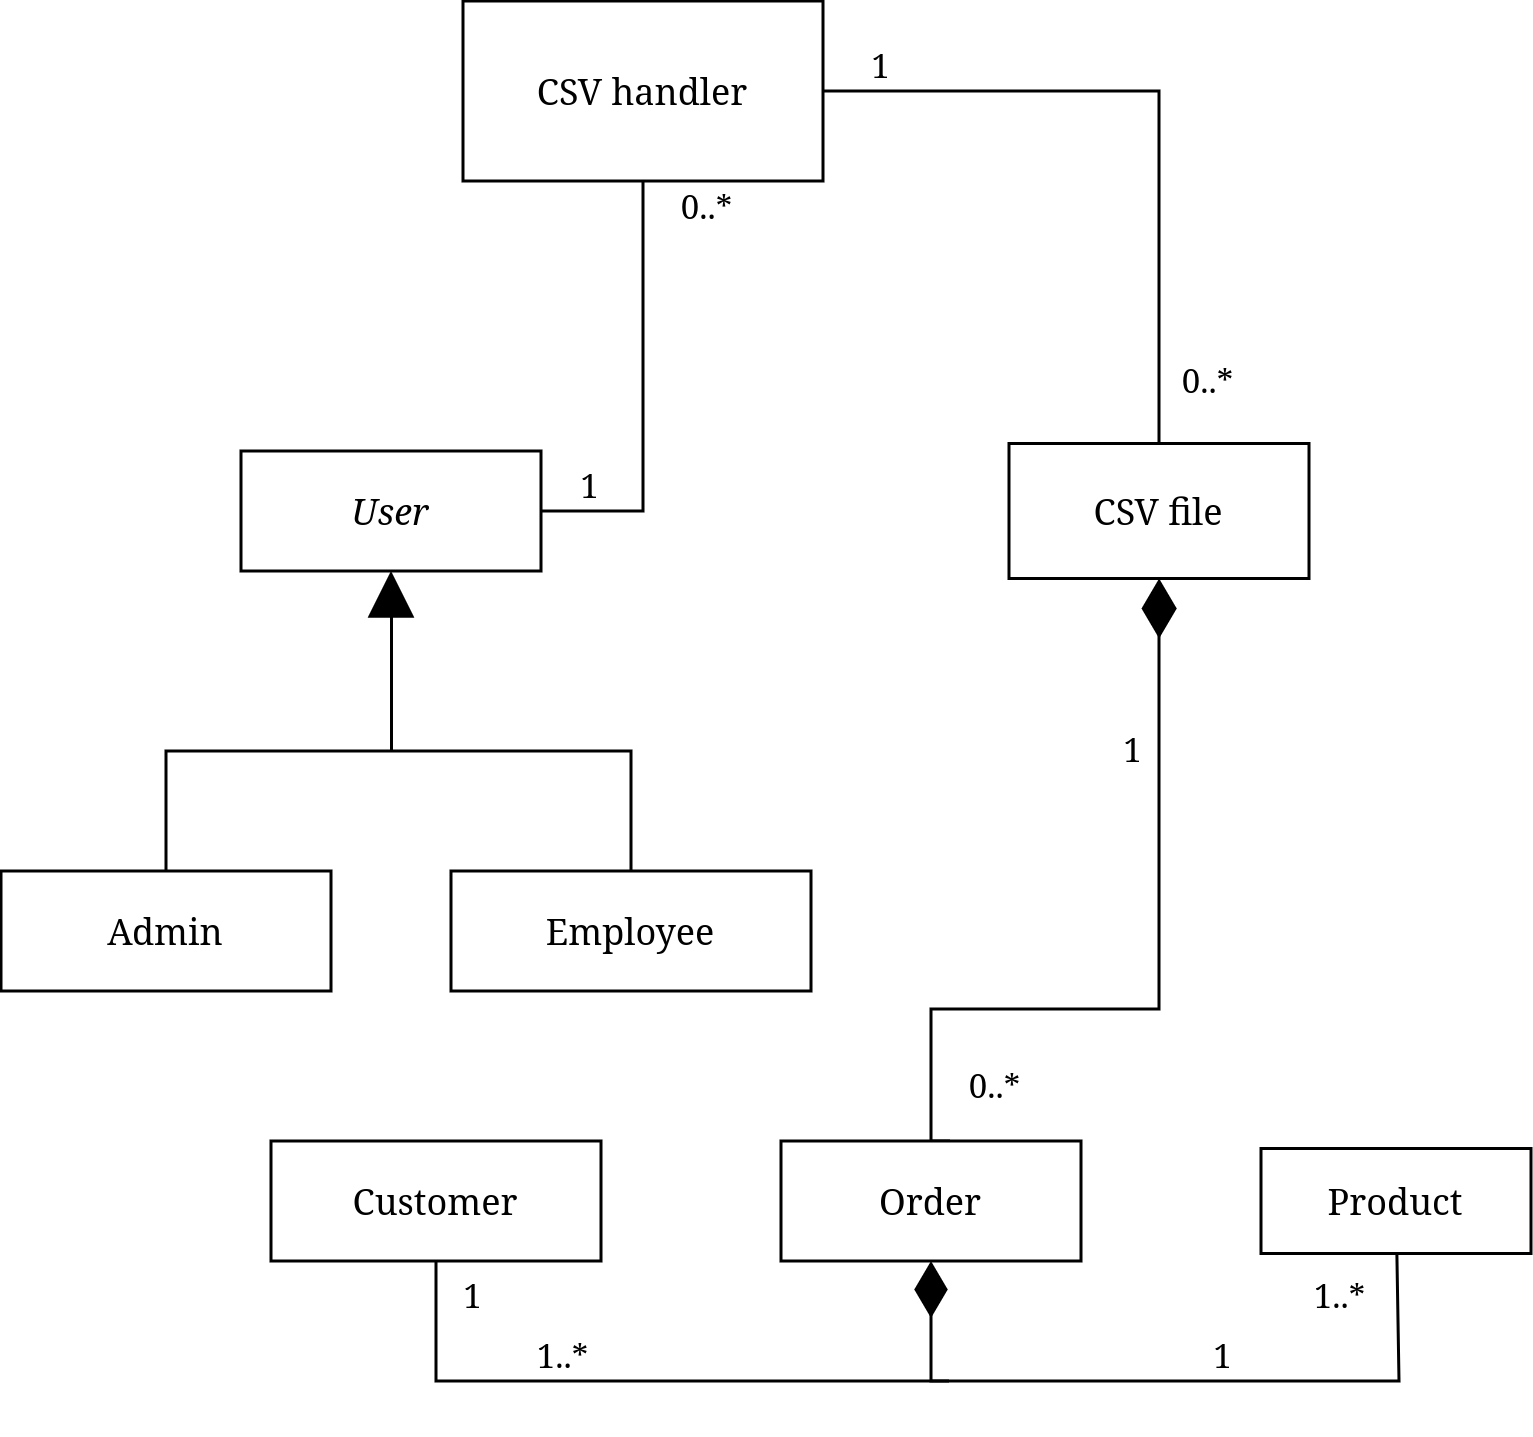
\includegraphics[scale=0.2]{class-overview}
    \caption{Class diagram of the problem domain.}\label{fig:pda-class-diagram}
\end{figure}
% textidote: ignore end

% textidote: ignore begin
\section{Event Table}\label{sec:event-table}
% textidote: ignore end

Multiple events were identified in the problem domain system.
An event represents one of the unique behaviors of one of the classes that were presented earlier in
Section~\ref{sec:classes-objects-and-structure}.

The event table that can be seen below in Table~\ref{tab:event-table}, visualizes the connections between all the
classes and events, and uses the ``updated'' even table model, as described by Mathiassen~\cite[102]{mathiassen2018}.

\newcommand{\rot}{\rotatebox{90}}
\newcolumntype{C}{>{\centering\arraybackslash}X}
\newcolumntype{g}{>{\columncolor[HTML]{aaaaaa}}c}

\begin{table}[H]
    \centering
    \begin{tabularx}{\textwidth}{ c p{4.5cm} C C C C C }
        & & \multicolumn{5}{ g }{Class} \\
        & & User & Admin (Owner) & Employee (Barista) & Order & Product
        \\
        \cmidrule{2-7}
        & Employed & & & + & &
        \\
        & Changed & & & \textasteriskcentered{} & &
        \\
        & Terminated & & & + & &
        \\
        & New order data available & & & & + &
        \\
        \rot{\rlap{~Event}}
        & Visualization viewed & \textasteriskcentered{} & \textasteriskcentered{} & \textasteriskcentered{}      & &
        \\
        & Product name mapped & & & & & \textasteriskcentered{}
        \\
        & Order data edited & & & & \textasteriskcentered{} &
        \\
        \cmidrule{2-7}
    \end{tabularx}
    \caption{The system's event table.
    \textbf{+} indicates that the event in question can occur zero or one time.
    \textbf{\textasteriskcentered{}} indicates it can occur zero or more times.}\label{tab:event-table}
\end{table}

